\section{Mockups}

In questa sezione vengono presentati i principali mockup dell’interfaccia utente di \textbf{JavaBrew}, la nostra applicazione dedicata alla gestione smart delle macchinette del caffè. Ogni mockup qui riportato mostra non solo il design grafico, ma anche le funzioni pratiche che i diversi tipi di utenti possono utilizzare. L’obiettivo è fornire un’anteprima chiara ed esaustiva dell’esperienza reale all’interno dell’app, dalla registrazione fino alle operazioni di amministrazione, manutenzione o acquisto.

\subsection{Login}
\begin{figure}[H]
    \centering
    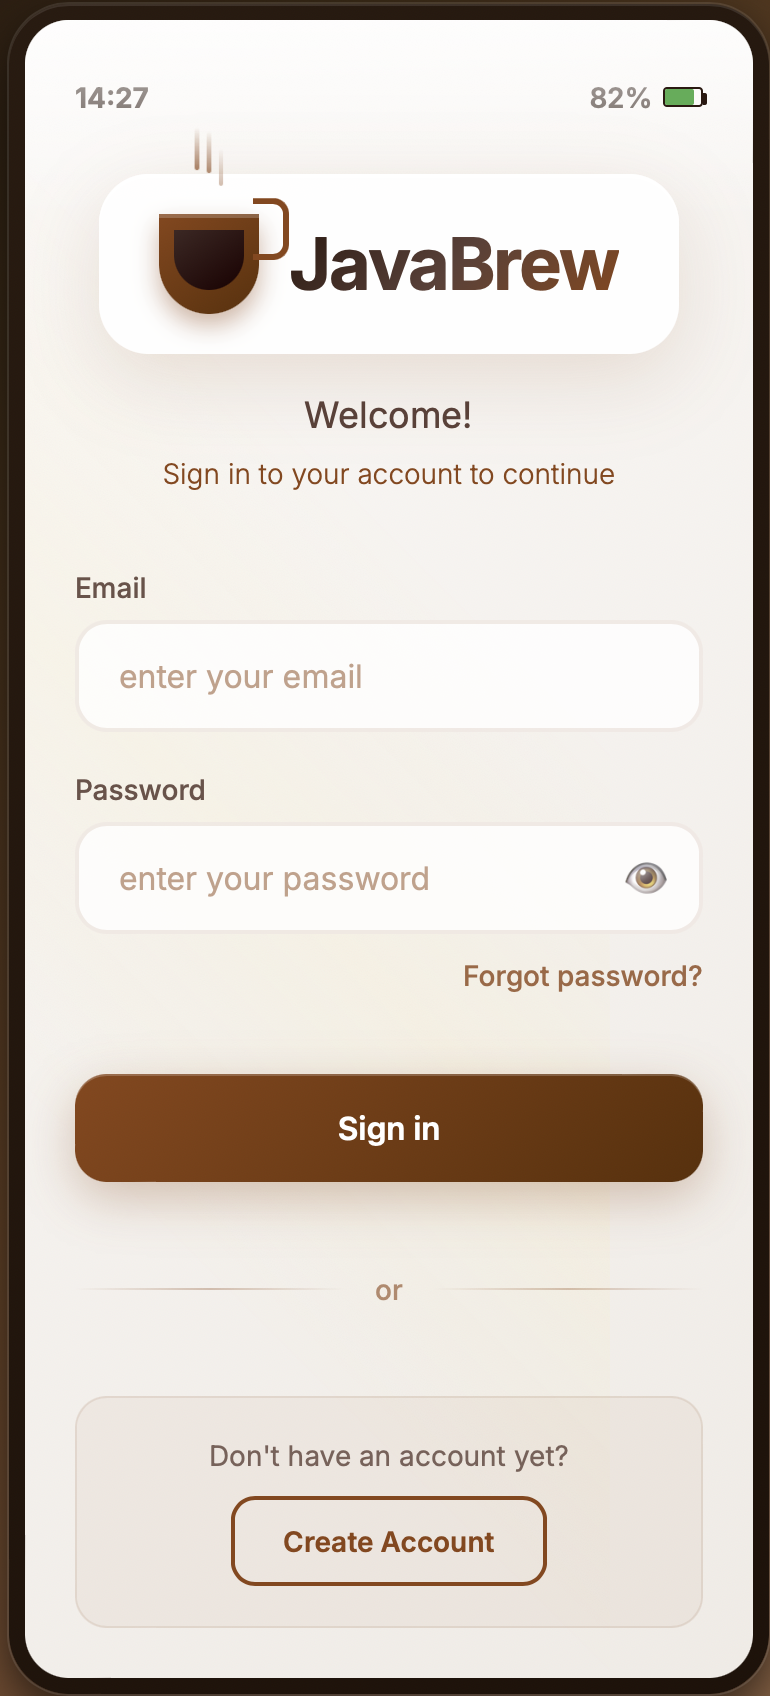
\includegraphics[width=0.5\textwidth]{./assets/login.png}
    \caption{Schermata di login.}
\end{figure}
La prima schermata che si incontra aprendo JavaBrew è la pagina di \textbf{login}, semplice ed essenziale. Qui l’utente inserisce la propria email e password per accedere all’account. È presente anche la funzione \emph{“Forgot password?”} per il recupero delle credenziali in caso di smarrimento. Per chi non avesse ancora un profilo, viene subito proposta la possibilità di crearne uno nuovo tramite il pulsante “Create Account”.

\subsection{Registrazione}
\begin{figure}[H]
    \centering
    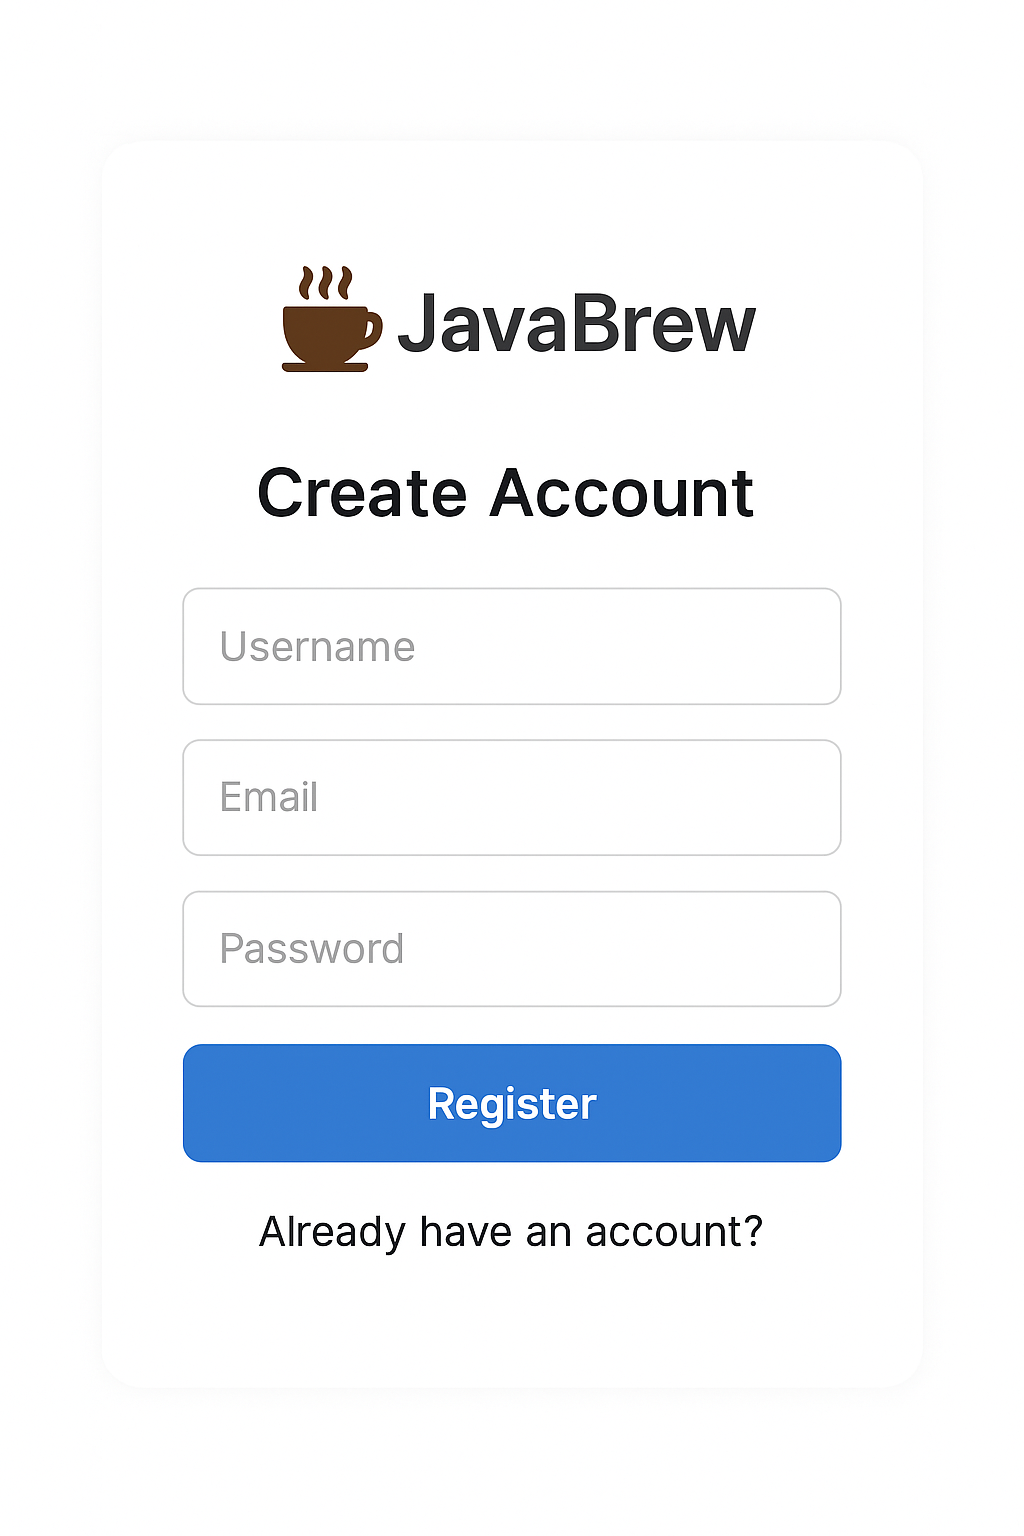
\includegraphics[width=0.5\textwidth]{./assets/Create_acoount.png}
    \caption{Schermata di registrazione.}
\end{figure}
Se l’utente sceglie di registrarsi, viene reindirizzato a una schermata molto intuitiva. In questa fase basta inserire email, scegliere una password e confermare i dati. Il processo di registrazione è stato progettato per essere il più veloce e trasparente possibile: bastano pochi click e si può subito iniziare a usare JavaBrew. Non manca la spunta obbligatoria per l’accettazione dei Termini di Servizio e della Privacy Policy, a tutela della sicurezza e della trasparenza.

\subsection{Dashboard Admin}
\begin{figure}[H]
    \centering
    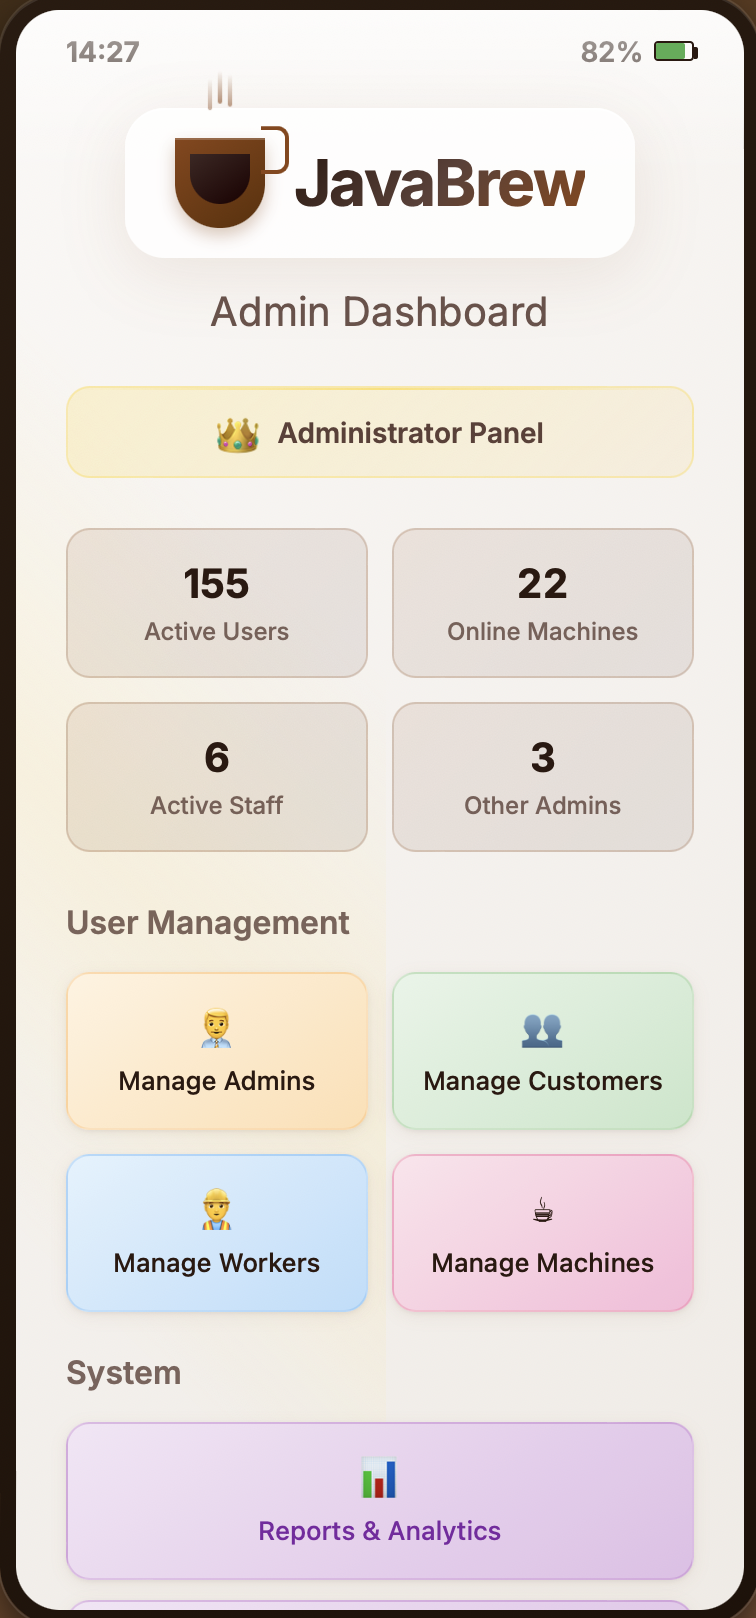
\includegraphics[width=0.5\textwidth]{./assets/admin.png}
    \caption{Dashboard amministratore.}
\end{figure}
Gli amministratori hanno accesso a una dashboard dedicata, ricca di informazioni e strumenti avanzati. Nella parte superiore si trovano subito le statistiche principali: numero di utenti attivi, macchinette online, staff operativo e altri amministratori. Sotto, il pannello di amministrazione è suddiviso in sezioni colorate e ben organizzate, per una gestione completa: dalla modifica e supervisione dei profili utente (admin, clienti, lavoratori) fino al controllo e alla configurazione delle macchine e dei prodotti disponibili. Inoltre, la sezione “Reports \& Analytics” consente di tenere sotto controllo le performance di vendita e il funzionamento generale del sistema in tempo reale.

\subsection{Customer Dashboard}
\begin{figure}[H]
    \centering
    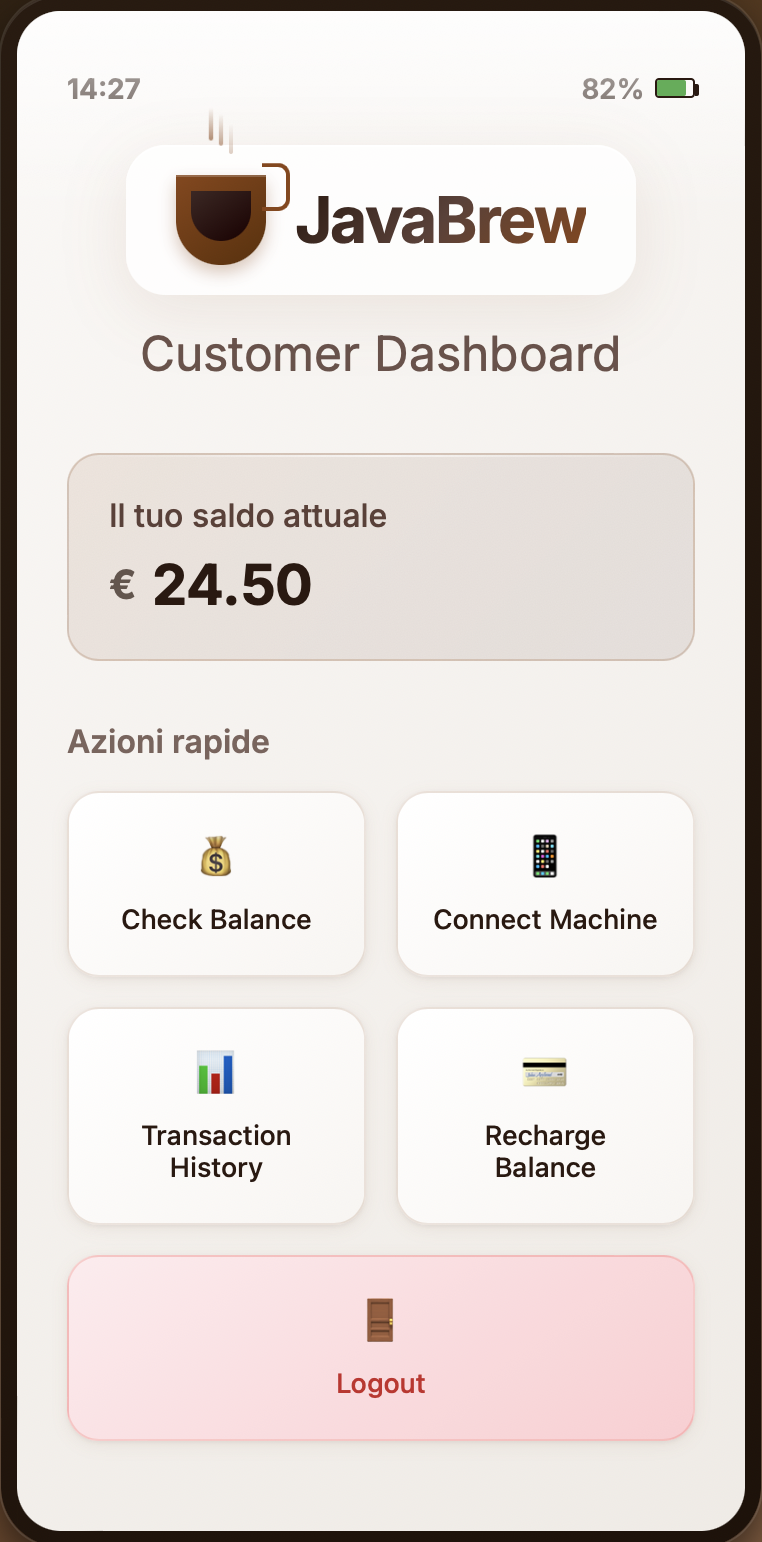
\includegraphics[width=0.4\textwidth]{./assets/customer.png}
    \caption{Dashboard utente standard (customer).}
\end{figure}
La dashboard per l’utente finale (customer) è pensata per offrire una gestione semplice del proprio saldo e delle operazioni principali. In alto, viene sempre mostrato il saldo attuale. Subito sotto, le azioni rapide permettono con un solo tap di consultare il saldo, collegare una macchinetta, controllare la cronologia delle transazioni oppure ricaricare il credito. L’interfaccia è essenziale, con pulsanti grandi e chiari per garantire un’esperienza piacevole anche agli utenti meno esperti.

\subsection{Worker Dashboard}
\begin{figure}[H]
    \centering
    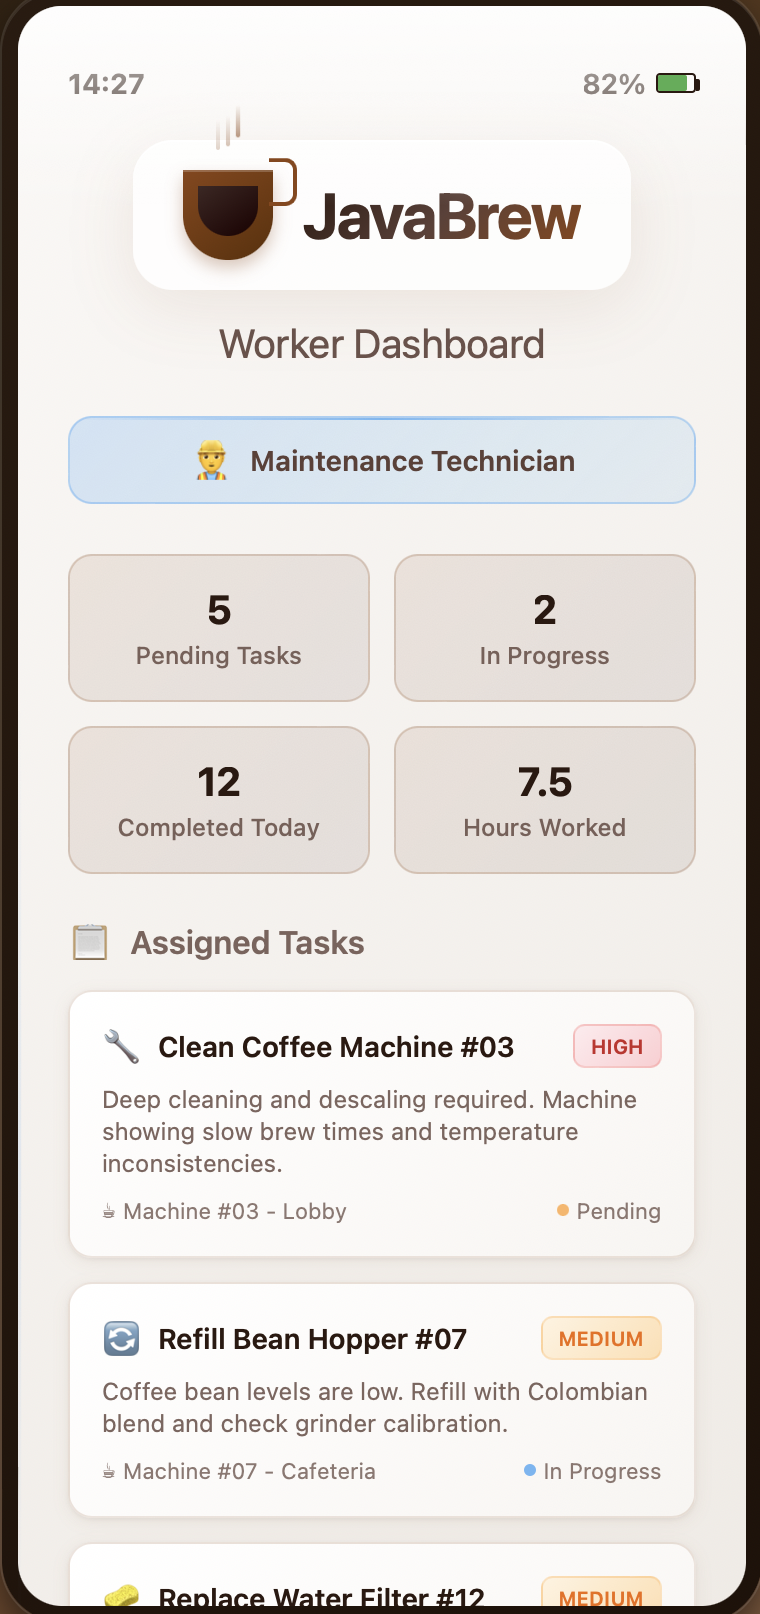
\includegraphics[width=0.4\textwidth]{./assets/worker.png}
    \caption{Dashboard per lavoratore.}
\end{figure}
Il lavoratore, o tecnico addetto alla manutenzione, trova nella propria dashboard tutte le informazioni operative di cui ha bisogno. La schermata mostra a colpo d’occhio il numero di task in sospeso, quelli in corso, il totale di attività completate e le ore lavorate nella giornata. Nella parte inferiore vengono elencati nel dettaglio tutti i compiti assegnati: ad esempio pulizia, ricarica dei chicchi o sostituzione di filtri, ognuno con priorità, descrizione e stato aggiornato in tempo reale. In questo modo la gestione della manutenzione diventa organizzata, trasparente e monitorabile.

\subsection{Items}
\begin{figure}[H]
    \centering
    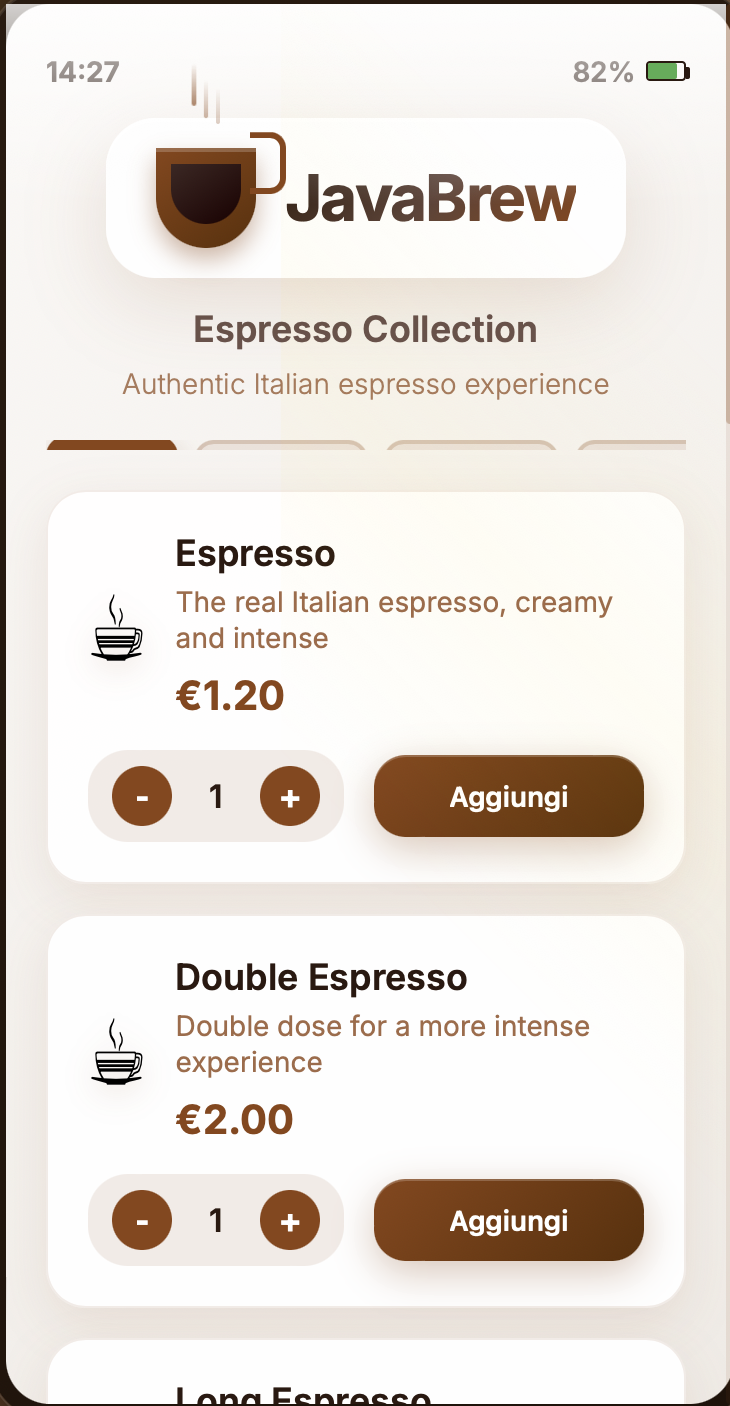
\includegraphics[width=0.4\textwidth]{./assets/items.png}
    \caption{Selezione prodotti e aggiunta al carrello.}
\end{figure}
Nella schermata degli articoli, ogni utente può vedere l’elenco dei prodotti disponibili (ad esempio espresso, doppio espresso, ecc.), ognuno con foto, descrizione, prezzo e possibilità di selezionare la quantità desiderata. In pochi secondi, grazie a una grafica intuitiva e moderna, è possibile aggiungere al carrello il proprio caffè preferito e completare l’acquisto direttamente dall’app.

\bigskip
Nel complesso, questi mockup mostrano un’interfaccia pensata per essere **user-friendly**, moderna ed estremamente funzionale. Ogni tipologia di utente (admin, lavoratore, customer) trova subito quello che cerca e può svolgere tutte le operazioni chiave in modo rapido, sicuro e intuitivo.
